\documentclass[12pt]{article}

\usepackage{sbc-template}
\usepackage{graphicx,url}
\usepackage[utf8]{inputenc}
\usepackage{multirow}
\usepackage{amsmath}

% O pacote babel para portugues esta quebrado nesta instalacao do TeX Live
% (opcoes 'brazil' e 'brazilian' falham), entao localizamos manualmente as
% palavras geradas automaticamente pelo LaTeX em vez de usar babel.
\renewcommand{\figurename}{Figura}
\renewcommand{\tablename}{Tabela}
\renewcommand{\refname}{Referências}

\sloppy

\title{1º Trabalho de Projeto e Análise de Algoritmos\\
  Escalonamento de Aulas via Transformar para Conquistar e Estratégia Gulosa}

\author{Gabriel Jared de Barros Amorim, Jonathan Santos Tadei,\\
  Lucas Ivanov Costa, Vinicius Eduardo Morais Oliveira}

\address{Colegiado de Ciência da Computação -- Universidade Estadual do Oeste do
  Paraná (UNIOESTE)\\
  Campus de Cascavel -- PR -- Brasil
  % TODO (grupo): inserir e-mails dos integrantes, ex.:
  % \email{nome1@aluno.unioeste.br, nome2@aluno.unioeste.br}
}

\begin{document}

\maketitle

\begin{abstract}
  This report compares two greedy solutions to the classroom-scheduling
  (interval partitioning) problem, under the Greedy Strategy and
  Transform-and-Conquer paradigms. The first solution (Greedy) applies the
  greedy room allocation directly on the original input order; the second
  (TCGreedy) sorts classes by start time before applying the very same
  greedy core. We present both a theoretical (asymptotic cost) and an
  empirical (measured running time over 28 input sizes, from 10 to
  1,000,000 classes) analysis, showing that although both solutions share
  the same $O(n^2)$ worst-case class, the sorting step yields a
  measurable practical gain beyond a certain input size.
\end{abstract}

\begin{resumo}
  Este trabalho compara duas soluções gulosas para o problema de
  escalonamento de aulas em salas (minimização do número de salas), sob os
  paradigmas Estratégia Gulosa e Transformar para Conquistar. A primeira
  solução (Greedy) aplica a alocação gulosa diretamente sobre a ordem
  original de entrada; a segunda (TCGreedy) ordena as aulas por horário de
  início antes de aplicar o mesmo núcleo guloso. São apresentadas as
  análises teórica (polinômios de custo assintótico) e prática (tempos de
  execução medidos empiricamente sobre 28 tamanhos de entrada, de 10 a
  1.000.000 aulas), mostrando que, apesar de ambas pertencerem à mesma
  classe de pior caso $O(n^2)$, a etapa de ordenação produz ganhos
  práticos mensuráveis a partir de um determinado tamanho de entrada.
\end{resumo}

\section{Introdução e Descrição do Problema}

O problema consiste em alocar $n$ aulas, cada uma com um horário de início e
término, ao menor número possível de salas, respeitando as seguintes
restrições:
\begin{itemize}
\item Duas aulas não podem ocupar a mesma sala no mesmo instante;
\item Não é necessário intervalo entre duas aulas consecutivas na mesma
  sala -- uma aula pode começar exatamente no instante em que a anterior
  termina.
\end{itemize}

Foram implementadas duas soluções gulosas que compartilham o mesmo núcleo
de alocação, diferindo apenas na etapa de pré-processamento da entrada:

\begin{itemize}
\item \textbf{Greedy}: processa as aulas na ordem original do arquivo de
  entrada;
\item \textbf{TCGreedy}: aplica a etapa de ``Transformar'' -- ordena as
  aulas por horário de início, de forma crescente -- e só então aplica o
  mesmo núcleo guloso.
\end{itemize}

Este problema é um caso clássico da literatura de algoritmos: corresponde
exatamente ao Exercício 16.1-4 de \cite{cormen:09}, apresentado logo após o
problema de seleção de atividades (Seção 16.1) como o problema de
\emph{escalonar atividades usando o menor número possível de salas de
conferência}. O próprio livro observa que esse problema equivale à
coloração de um grafo de intervalos (cada aula é um vértice, e duas aulas
incompatíveis -- que se sobrepõem -- são ligadas por uma aresta): o número
mínimo de salas necessárias é igual ao número cromático desse grafo, que
por sua vez é igual à \emph{profundidade máxima} de sobreposição
simultânea de aulas (o maior número de aulas ativas ao mesmo tempo, em
qualquer instante). O mesmo problema -- com a mesma função de seleção
usada pelo TCGreedy, ``selecionar a aula com o menor tempo de início'' --
também é apresentado no material da disciplina, na seção ``Escalonamento
de Tarefas'' \cite{brun:26}.

\section{Descrição das Soluções}

\subsection{Núcleo Guloso Compartilhado}
\label{sec:nucleo}

O núcleo, doravante chamado \texttt{alocarSalas}, mantém uma lista de salas
abertas, cada uma com o horário de término da última aula alocada nela.
Para cada aula, na ordem em que é processada:

\begin{enumerate}
\item Percorre as salas já abertas em busca da primeira cujo horário de
  término seja menor ou igual ao horário de início da aula atual
  (\textit{first-fit});
\item Se encontrar, reutiliza essa sala, atualizando seu horário de
  término;
\item Caso contrário, abre uma nova sala para a aula atual.
\end{enumerate}

\begin{verbatim}
alocarSalas(aulas):
    terminoDaSala = []
    para cada aula em aulas:
        sala = procurar em terminoDaSala uma sala com
               termino <= aula.inicio
        se encontrou:
            atualizar termino dessa sala para aula.termino
        senao:
            abrir nova sala com termino = aula.termino
    retornar numero de salas abertas
\end{verbatim}

\subsection{Greedy}

Aplica \texttt{alocarSalas} diretamente sobre o vetor de entrada, sem
qualquer ordenação prévia.

\subsection{TCGreedy}

Ordena o vetor de aulas por horário de início ($O(n \log n)$) e em seguida
aplica a \textbf{mesma} função \texttt{alocarSalas} usada pelo Greedy. A
única diferença entre as duas soluções está, portanto, na ordem em que as
aulas chegam ao núcleo guloso. Essa combinação de ordenação por início
seguida de alocação gulosa corresponde exatamente ao algoritmo de
escalonamento apresentado em aula \cite{brun:26}, cuja função de seleção é
``selecionar a tarefa com o menor tempo de início''.

\section{Análise de Complexidade Assintótica}
\label{sec:complexidade}

\subsection{Modelo de custo}

Seguindo o método de contagem de operações básicas apresentado em aula
(atribuição, teste lógico, incremento, indexação, soma e retorno como
operações de custo unitário; o tempo de uma sequência de comandos é o
maior tempo de qualquer comando da sequência; o tempo de comandos
aninhados é obtido pelo produto/soma das complexidades), reescrevemos o
núcleo \texttt{alocarSalas} (Seção~\ref{sec:nucleo}) com laços indexados,
equivalentes ao \texttt{for-each} usado na implementação em Java:

\begin{verbatim}
1   terminoDaSala = novo vetor de tamanho n
2   numSalas = 0
3   operacoes = 0
4   for (i = 0; i < n; i++)
5       salaEscolhida = -1
6       for (s = 0; s < numSalas; s++)
7           operacoes = operacoes + 1
8           if (terminoDaSala[s] <= aulas[i].inicio)
9               salaEscolhida = s
10              break
11      if (salaEscolhida == -1)
12          salaEscolhida = numSalas
13          numSalas = numSalas + 1
14      terminoDaSala[salaEscolhida] = aulas[i].termino
15  retornar numSalas, operacoes
\end{verbatim}

\subsection{Núcleo guloso -- pior caso (comum às duas soluções)}

O pior caso ocorre quando a condição da linha 8 nunca é verdadeira --
por exemplo, quando as $n$ aulas se sobrepõem todas mutuamente
(compartilham um mesmo instante em comum). Nesse cenário, o laço interno
nunca encontra sala livre: roda até o fim sem \texttt{break} (linhas
9--10 nunca executam) e o \texttt{if} da linha 11 é sempre verdadeiro
(sempre abre sala nova). Quando o laço da linha 6 começa a executar para
a $i$-ésima aula ($i = 0, \dots, n-1$), o valor de \texttt{numSalas}
naquele momento é exatamente $i$, pois uma sala nova foi aberta em cada
uma das $i$ iterações anteriores. Isso caracteriza um \textbf{laço
aninhado dependente}: o limite do laço interno cresce junto com o
índice do laço externo, de forma análoga ao exemplo de laços
dependentes visto em aula -- e por isso seu custo total é obtido somando
uma progressão aritmética.

A Tabela~\ref{tab:custo-nucleo} detalha o custo de cada linha.

\begin{table}[ht]
\centering
\footnotesize
\caption{Custo do núcleo \texttt{alocarSalas} no pior caso, linha a linha.}
\label{tab:custo-nucleo}
\begin{tabular}{c|l|l|l}
\hline
\textbf{Linha} & \textbf{Custo/execução} & \textbf{Nº de execuções} & \textbf{Total} \\
\hline
1  & $n$ (alocação/zeragem) & 1 & $n$ \\
2  & 1 atrib. & 1 & $1$ \\
3  & 1 atrib. & 1 & $1$ \\
4  & $1$ atrib. $+ n(\text{tlog}+\text{incr}) + \text{tlog}$ & 1 & $2n+2$ \\
5  & 1 atrib. & $n$ vezes & $n$ \\
6  & $1$ atrib. $+ i(\text{tlog}+\text{incr}) + \text{tlog}$ & $\sum_{i=0}^{n-1}$, numSalas$=i$ & $n^2+n$ \\
7  & 1 atrib. & $\sum_{i=0}^{n-1} i$ & $\frac{n^2-n}{2}$ \\
8  & 1 tlog & $\sum_{i=0}^{n-1} i$ & $\frac{n^2-n}{2}$ \\
9--10 & -- & pior caso: nunca executa & $0$ \\
11 & 1 tlog & $n$ vezes & $n$ \\
12--13 & 2 atrib. & $n$ vezes (sempre verd.) & $2n$ \\
14 & 1 index $+$ 1 atrib. & $n$ vezes & $2n$ \\
15 & 1 retorno & 1 & $O(1)$ \\
\hline
\end{tabular}
\end{table}

Somando todas as linhas:

\begin{equation}
T_{nucleo}(n) = n + 1 + 1 + (2n+2) + n + (n^2+n) + \frac{n^2-n}{2} + \frac{n^2-n}{2} + n + 2n + 2n + O(1)
\end{equation}

\begin{equation}
T_{nucleo}(n) = 2n^2 + 9n + O(1) \in \Theta(n^2)
\end{equation}

ou seja, $O(n^2)$ no pior caso.

\subsection{Greedy}

O Greedy aplica apenas o núcleo, diretamente sobre a entrada, sem custo
adicional:

\begin{equation}
T_{Greedy}(n) = T_{nucleo}(n) = 2n^2 + 9n + O(1) \in O(n^2)
\end{equation}

\subsection{TCGreedy}

O TCGreedy soma ao núcleo o custo da ordenação por horário de início,
tratada como uma chamada de função de complexidade conhecida (assim como
funções puras vistas em aula, ex. $raiz(n)$, $potencia(base,expoente)$).
O método \texttt{Arrays.sort} usado para ordenar um vetor de objetos
(como \texttt{Aula[]}) implementa uma variante estável de \textit{merge
sort} (TimSort), cujo número de comparações no pior caso é
$T_{sort}(n) = n\log_2 n$. Logo:

\begin{equation}
T_{TCGreedy}(n) = T_{sort}(n) + T_{nucleo}(n) = n\log_2 n + 2n^2 + 9n + O(1) \in O(n^2)
\end{equation}

pois o termo quadrático domina o termo $n \log n$ para $n$ suficientemente
grande.

\subsection{Consequência teórica}

\textbf{As duas soluções pertencem à mesma classe assintótica de pior
caso, $O(n^2)$}, já que compartilham o mesmo núcleo de alocação -- o
termo $n \log n$ adicional do TCGreedy é absorvido pelo termo quadrático
que domina em ambos os polinômios. A diferença entre as soluções não
aparece na classe assintótica de pior caso, mas sim (a) no comportamento
médio prático e (b) na qualidade da solução (número de salas), como
discutido na Seção~\ref{sec:resultados}.

\section{Metodologia Experimental}
\label{sec:metodologia}

\subsection{Configuração da Máquina de Testes}

\begin{itemize}
\item \textbf{Sistema operacional:} Arch Linux, kernel 7.1.3-arch1-3;
\item \textbf{Processador:} Intel(R) Core(TM) i5-8265U CPU @ 1.60GHz
  (4 núcleos / 8 threads);
\item \textbf{Memória RAM:} 7,6 GiB;
\item \textbf{Linguagem/\textit{runtime}:} Java (OpenJDK 21.0.11);
\item \textbf{IDE:} nenhuma -- compilação e execução via linha de
  comando (terminal), sem uso de ambiente de desenvolvimento integrado;
\item \textbf{Compilação:} \texttt{javac}, sem \textit{flags} de
  otimização especiais;
\item \textbf{Execução:} \texttt{java -cp out BenchmarkRunner
  <pasta-entradas> <csv-saida> <timeout>}.
\end{itemize}

\subsection{Processo de Coleta dos Tempos}

Para cada um dos tamanhos de entrada disponibilizados e para cada
estratégia:

\begin{enumerate}
\item A entrada é lida uma única vez -- a leitura do arquivo \textbf{não}
  entra na medição de tempo;
\item O núcleo guloso é executado 6 vezes sobre os mesmos dados em
  memória, cronometrado com \texttt{System.nanoTime()};
\item A primeira execução é descartada (aquecimento de JIT);
\item Calcula-se a média das 5 execuções restantes;
\item São também registrados, por execução, o número de salas resultante
  e o número de operações de comparação do núcleo guloso (variáveis de
  interesse);
\item O \texttt{BenchmarkRunner} suporta um orçamento de tempo opcional
  por execução (parametrizável ou totalmente desligável), pensado para
  evitar que uma entrada muito grande trave o benchmark indefinidamente.
  A coleta final apresentada neste relatório foi feita com esse orçamento
  \textbf{desligado}, para obter tempos reais mesmo nos tamanhos maiores
  -- o maior tempo médio observado foi o do Greedy em $n=1.000.000$,
  $\sim$121,1s por execução.
\end{enumerate}

Os dados brutos estão disponíveis em \texttt{resultados/tempos.csv}, no
repositório de código-fonte que acompanha este relatório.

\section{Resultados}
\label{sec:resultados}

A Figura~\ref{fig:linear} mostra o tempo médio de execução em função do
tamanho da entrada, em escala linear; a Figura~\ref{fig:loglog} mostra os
mesmos dados em escala log-log, que evidencia melhor o comportamento nas
ordens de grandeza menores. A Tabela~\ref{tab:resultados} resume os
valores medidos para tamanhos representativos.

\begin{figure}[ht]
\centering
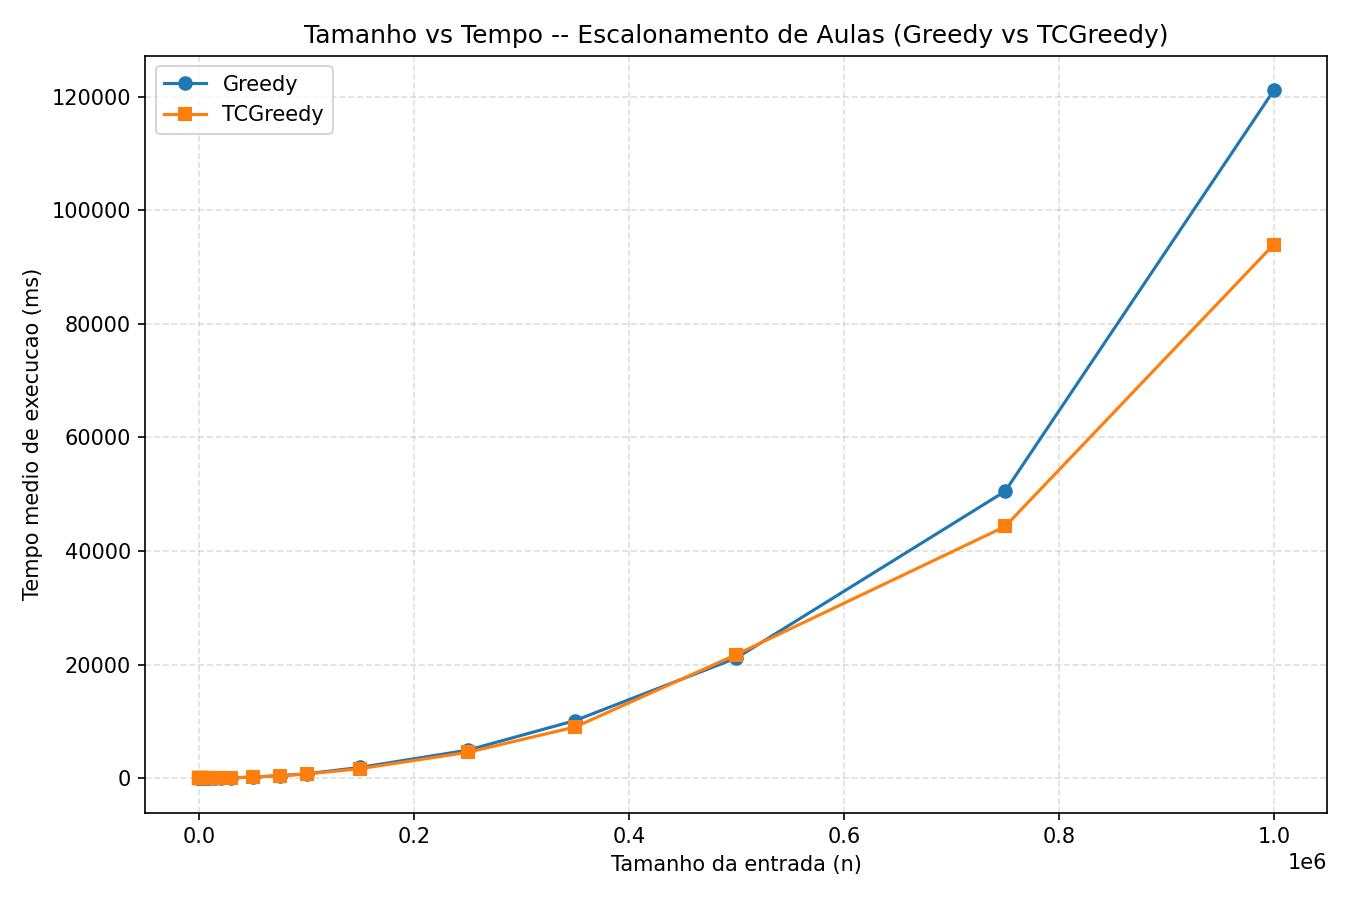
\includegraphics[width=.8\textwidth]{tamanho_vs_tempo_linear.png}
\caption{Tamanho vs. tempo médio de execução (ms) -- escala linear.}
\label{fig:linear}
\end{figure}

\begin{figure}[ht]
\centering
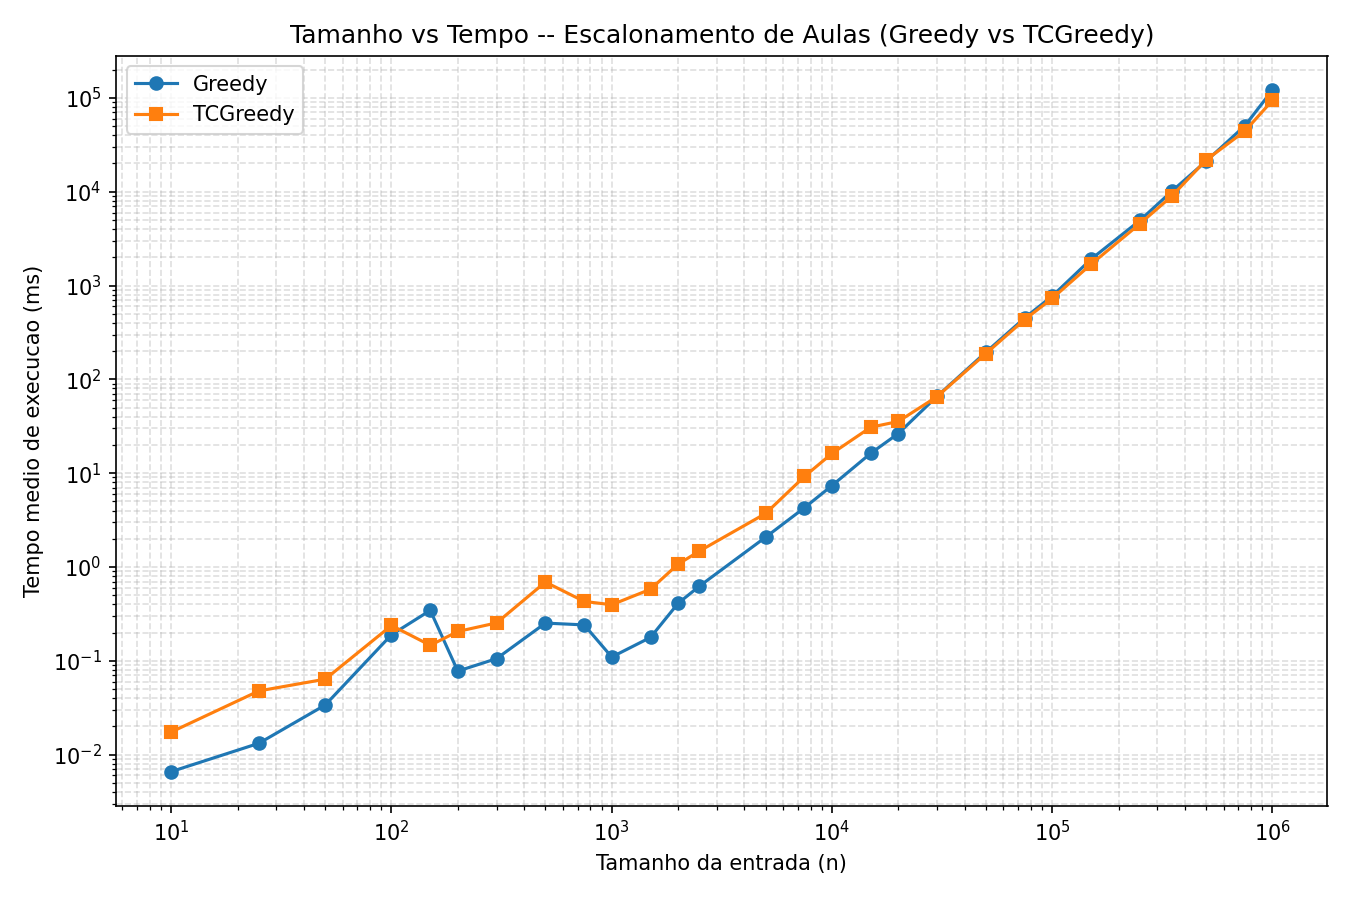
\includegraphics[width=.8\textwidth]{tamanho_vs_tempo_log_log.png}
\caption{Tamanho vs. tempo médio de execução (ms) -- escala log-log.}
\label{fig:loglog}
\end{figure}

\begin{table}[ht]
\centering
\caption{Tempo médio de execução (ms) e número de salas usadas, para
  tamanhos de entrada representativos (todos os valores são média de 5
  execuções, sem interrupção por tempo).}
\label{tab:resultados}
\begin{tabular}{r|rr|rr}
\hline
\multirow{2}{*}{$n$} & \multicolumn{2}{c|}{Tempo médio (ms)} & \multicolumn{2}{c}{Salas usadas} \\
 & Greedy & TCGreedy & Greedy & TCGreedy \\
\hline
10      & 0,007      & 0,017      & 7       & 7       \\
100     & 0,190      & 0,238      & 62      & 53      \\
1.000   & 0,110      & 0,396      & 531     & 481     \\
10.000  & 7,373      & 16,222     & 4.576   & 4.405   \\
20.000  & 26,452     & 35,551     & 9.703   & 9.606   \\
30.000  & 65,945     & 65,458     & 13.234  & 12.864  \\
50.000  & 194,644    & 188,233    & 25.313  & 25.090  \\
100.000 & 770,891    & 727,892    & 50.402  & 49.979  \\
150.000 & 1.905,461  & 1.681,344  & 75.314  & 74.868  \\
250.000 & 4.934,210  & 4.551,336  & 125.691 & 124.877 \\
350.000 & 10.156,943 & 9.018,185  & 175.876 & 175.219 \\
500.000 & 21.163,517 & 21.774,828 & 251.179 & 250.175 \\
750.000 & 50.509,619 & 44.313,597 & 376.653 & 375.352 \\
1.000.000 & 121.092,902 & 93.954,894 & 642.836 & 642.819 \\
\hline
\end{tabular}
\end{table}

Principais observações:

\begin{itemize}
\item \textbf{Número de salas} cresce de forma aproximadamente linear com
  $n$ em ambas as soluções (ex.: $n=250.000 \rightarrow$ 125.691 salas no
  Greedy, 124.877 no TCGreedy; $n=1.000.000 \rightarrow$ 642.836 no
  Greedy, 642.819 no TCGreedy), confirmando que o núcleo guloso de fato se
  comporta como $O(n^2)$ na prática, não apenas no pior caso teórico, já
  que o número de salas abertas $r$ é proporcional a $n$;
\item \textbf{TCGreedy realiza menos operações} de comparação no núcleo
  guloso do que Greedy, e resulta em \textbf{menos ou o mesmo número de
  salas} (qualidade de solução igual ou melhor), para todos os tamanhos
  testados -- a ordenação por início ajuda o \textit{first-fit} a
  encontrar salas livres mais cedo, em média, e evita alocações
  desnecessárias;
\item \textbf{Ponto de cruzamento no tempo de parede:} para $n$ pequeno
  (até $\sim$20.000), o Greedy é mais rápido em tempo de parede, pois o
  custo constante do \texttt{Arrays.sort} supera a economia de operações
  do núcleo (ex.: $n=20.000 \rightarrow$ Greedy 26,5ms vs TCGreedy
  35,6ms). A partir de $n\approx$30.000, esse quadro se inverte -- o
  TCGreedy passa a ser mais rápido na maioria dos tamanhos maiores (ex.:
  $n=30.000 \rightarrow$ Greedy 65,9ms vs TCGreedy 65,5ms; $n=1.000.000
  \rightarrow$ Greedy 121.092,9ms vs TCGreedy 93.954,9ms), pois o custo
  $O(n \log n)$ do \textit{sort} passa a ser irrelevante frente à
  economia de operações $O(n^2)$ do núcleo. Há uma inversão pontual em
  $n=500.000$ (Greedy 21.163,5ms vs TCGreedy 21.774,8ms), provavelmente
  causada por ruído de medição (pausas de \textit{garbage collector} ou
  variação de carga do sistema) e não por uma mudança real de
  comportamento algorítmico, já que a tendência volta a favorecer o
  TCGreedy nos dois tamanhos seguintes.
\end{itemize}

\section{Análise Crítica}

As duas soluções compartilham exatamente o mesmo núcleo guloso e, por
isso, pertencem à mesma classe assintótica de pior caso, $O(n^2)$ -- a
etapa de ``Transformar'' (ordenação, $O(n \log n)$) não muda essa classe,
pois o núcleo domina o crescimento assintótico. Isso ficou evidente na
prática: o número de operações e o número de salas crescem de forma
consistente com $n^2$ nas duas soluções.

Ainda assim, o ``Transformar'' tem um efeito prático real e mensurável,
mesmo sem mudar a classe assintótica de pior caso:

\begin{itemize}
\item Ele \textbf{reduz a constante multiplicativa} do núcleo $O(n^2)$
  (menos operações por aula, em média, porque salas livres são
  encontradas mais cedo);
\item Ele \textbf{melhora a qualidade da solução} (menos salas usadas) --
  um benefício que nem chega a ser exigido nos critérios formais deste
  trabalho, mas é um efeito colateral positivo interessante do
  pré-processamento;
\item Ele \textbf{adiciona um custo fixo} (o \textit{sort} em si), que só
  compensa a partir de um tamanho de entrada onde a economia de operações
  do núcleo supera esse custo -- daí o ponto de cruzamento observado por
  volta de $n\approx$20.000--30.000.
\end{itemize}

A melhora na qualidade da solução (item anterior) não é uma coincidência
empírica, mas consequência direta da teoria de coloração de grafos de
intervalos discutida na Seção~\ref{sec:complexidade} \cite{cormen:09}: o
número mínimo de salas necessárias é igual à profundidade máxima de
sobreposição simultânea de aulas, e processar as aulas em ordem crescente
de horário de início, alocando cada uma à primeira sala livre disponível
-- exatamente o que o TCGreedy faz -- é conhecido por atingir esse mínimo
teórico. Já o Greedy processa as aulas na ordem arbitrária do arquivo de
entrada, sem essa garantia: uma aula que começa cedo mas aparece tarde no
arquivo pode ser processada depois de aulas que começam mais tarde,
fazendo com que o algoritmo abra salas que uma aula ainda não processada
poderia ter reaproveitado. É por isso que o TCGreedy iguala ou usa menos
salas que o Greedy em \textbf{todos} os tamanhos testados, nunca o
contrário.

Esse resultado ilustra bem o princípio geral do paradigma Transformar
para Conquistar \cite{levitin:11}: pré-processar a entrada não
necessariamente melhora a complexidade assintótica de pior caso do
algoritmo seguinte, mas pode melhorar substancialmente o comportamento
médio/prático -- e o ganho só se manifesta quando a etapa de
``Conquistar'' de fato tira proveito da transformação (aqui, o
\textit{first-fit} tira proveito de estar processando aulas em ordem
crescente de início, mesmo sem ter sido redesenhado para isso).

Os tempos observados em $n=1.000.000$ (a maior entrada testada -- Greedy
121,09s, TCGreedy 93,95s por execução) reforçam, na prática, por que
algoritmos $O(n^2)$ \cite{cormen:09} são considerados proibitivos para
entradas grandes: cada execução isolada já leva mais de um minuto, mesmo
em um processador moderno.

\section{Conclusão}

O experimento mostrou que, embora Greedy e TCGreedy compartilhem o mesmo
núcleo de alocação e por isso tenham a mesma classe assintótica de pior
caso ($O(n^2)$), a etapa de pré-ordenação do TCGreedy tem impacto prático
real: reduz o número de operações do núcleo e iguala ou reduz o número de
salas usadas em todos os tamanhos testados, e passa a compensar seu
próprio custo (o \textit{sort}) a partir de $n\approx$20.000--30.000,
tornando-se a solução mais rápida em tempo de parede na maior parte dos
tamanhos maiores testados (com uma única inversão pontual em
$n=500.000$, provavelmente ruído de medição). Isso confirma que o valor
do paradigma Transformar para Conquistar não está necessariamente em
mudar a ordem de complexidade assintótica, mas em explorar uma estrutura
na entrada (aqui, a ordem cronológica das aulas) que barateia o
comportamento médio do algoritmo que vem em seguida. Os tempos crescentes
nas entradas maiores testadas (chegando a mais de um minuto por execução
em $n=1.000.000$) também evidenciaram, de forma concreta, por que
algoritmos $O(n^2)$ se tornam inviáveis à medida que $n$ cresce.

\section{Código-fonte}

O código-fonte completo está disponível na pasta \texttt{src/} do
repositório deste trabalho, incluindo os comandos de medição de tempo
(\texttt{System.nanoTime()}) e contagem de operações
(\texttt{EscalonadorGuloso.Resultado.operacoes()}).

\bibliographystyle{sbc}
\bibliography{sbc-template}

\end{document}
